\section{Approach}
\label{sec:approach}
Our new ext-abs framework is illustrated in \figref{fig:overview}.
There are three main components: a keyword-based extractor,
an abstractor and a comprehensively rewarded reinforcement learning (RL). 
%Given a source document, at first, the extractor is trained to extract set-level pseudo summary,
%and the abstractor is trained 
%Then the abstractor parallelly summarizes each set of sentences in pseudo summary 
%and concatenate the summarized sentences as the final abstractive summary.
%In this way, the input to the abstractor is much shorter than original source document which alleviate required GPU memories, and process each set in parallel can save time.
As a preprocessing step, we first obtain the set-level pseudo 
summary from the training data.
We then pretrain the keyword-based extractor using the source document
and the pseudo summary, and 
the parallel abstractor using the pseudo summary and
the reference summary.
Finally, we use RL to bridge the pretrained extractor and 
abstractor to further finetune the parameters in both models. 
The RL updates the extractor and abstractor by a comprehensive reward 
evaluating both the extracted intermediate summaries and abstractive summaries 
at sentence-level, set-level and summary-level.

%\JQ{add the input and output between each components of the model especially the intuition? }
%\YZ{Extractor-Abstractor Framework: Figure of the framework}
\begin{figure*}[th]
    \centering
    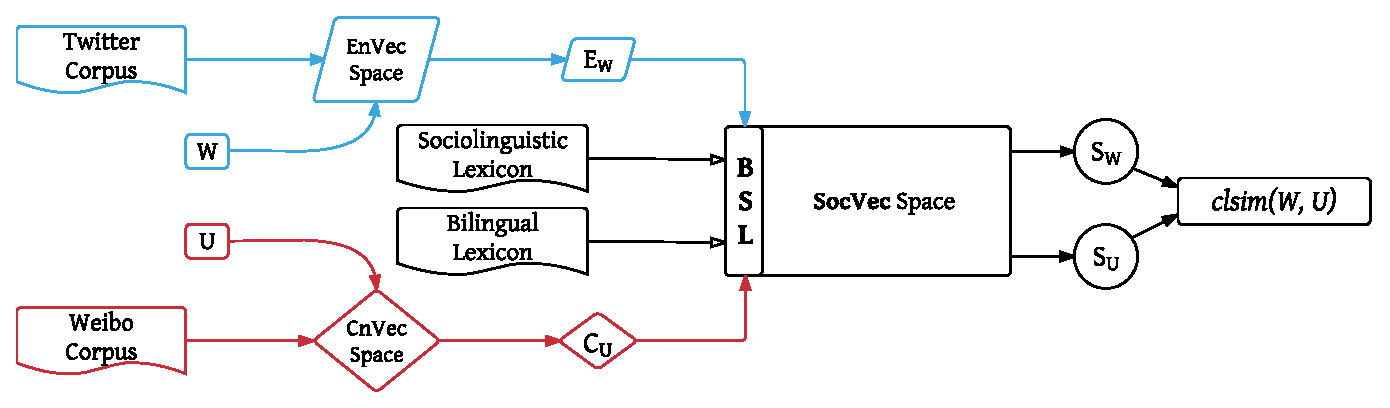
\includegraphics[width=0.85\linewidth]{overview}
    \caption{The overview of keyword-aware reinforced extractor-abstractor framework. }
    \label{fig:overview}
\end{figure*}


In the rest of this paper, we use the following definitions.
\begin{itemize}
\item A source document $D$ is a sequence of sentences 
$(d_0, ...,d_i,...)$; 
\item A set-level \textit{pseudo summary} $P$ is
a sequence of sentences organized in sets 
denoted as $(p^0_0, p^0_1,...,p^l_i,...,p^m_x)$ 
where $p_i^l$ is the $i^{th}$ sentence in the sequence that
belongs to the $l^{th}$ set;
\item The output of extractor, i.e.,  \textit{intermediate summary}
$Q$, is a sequence of sentences denoted as 
($q^0_0$, $q^0_1$,..., $q^l_i$,..., $q^M_y$) similar to $P$;
%To be consistent with the Algorithm \ref{alg:alg},
\item A \textit{reference summary} $R$ consists of sentences 
($r_0$, $r_1$,..., $r_i$,..., $r_z$);
\item A \textit{reorganized reference summary} $\hat{R}$ consists of sentences 
($\hat{r}^0_0$, $\hat{r}^0_1$,..., $\hat{r}^l_i$,..., $\hat{r}^m_z$), 
similar to $P$ and $Q$; 
\item The generated abstractive summary $A$ is a sequence of sentence 
$(a^0,a^1,...,a^l,...,a^{M})$ and $a$ denotes the set of sentences.
%$p^l_i$ means that the $i$-th sentence in summary $P$ belongs to the $l$-th sets.
%The $i$ means the index of the sentence.
%The sentence with $l$ means that this sentence belongs to the $l$-th multi-sentence set.
\item $t$ ranges over the time steps in both encoding and decoding.
\end{itemize}

Next, we describe the preprocessing of the training data 
to obtain pseudo summaries,
and the key components in the framework.~\footnote{Our framework is flexible with respect to the choice of document encoder and abstractor.}
\cut{%%%%%%%
The main notations used in our approach are shown in \tabref{tab:notation}.
\begin{table}[th]
    \small
	\centering
	\begin{tabular}{|l|l|}
		\hline
		Notation & Description \\ \hline
	    \hline
		$D=(d_0,d_1,...)$ & \tabincell{l}{Source document. $d_i$ is the $i$-th sentence in $D$.}\\
		\hline
		$R=(r_0,r_1,...)$ & \tabincell{l}{Reference summary. $r_i$ is the $i$-th sentence in $R$.}\\
		\hline
		$K=(k^0_0,k^0_1,...,k^i_j)$ & \tabincell{l}{Keywords in reference summary. \\ $k^i$ is the keywords in $r_i$.\\
		                                           $k_j$ is the $j$-th keyword in $K$}.\\
		\hline
		$P=(p^0_0,p^0_1,...,p^i_j,...)$ & \tabincell{l}{Pseudo summary. \\ $p^i$ is the $i$-th set of sentences in $P$.\\
		                                           $p_j$ is the $j$-th sentence in $K$}.\\
		%$P=(p_0,p_1,...)$ & \tabincell{l}{Pseudo summary. $p_i$ is the $i$-th set of sentences in $P$.}\\
		\hline
		$\hat{R}=(\hat{r}^0_0,\hat{r}^0_1,...,\hat{r}^i_j,...)$ & \tabincell{l}{Pseudo summary. \\ $\hat{r}^i$ is the $i$-th set of sentences in $\hat{R}$.\\
		                                           $\hat{r}_j$ is the $j$-th sentence in $\hat{R}$}.\\
		%$\hat{R}=(\hat{r},\hat{r}_1,...)$ & \tabincell{l}{Merged reference summary. \\ $m_i$ is the $i$-th set of sentences in $M$.}\\
		\hline
	\end{tabular}
    \caption{The notation}
    
\end{table}
}%%%%%%%%%%

\subsection{Data Pre-processing: Set-level Matching Heuristics}
\label{sec:preprocess}
%The ext-abs framework first uses extractor to obtain the pseudo 
%summary, followed by using abstractor to paraphrase
%the pseudo summary to generate an abstractive summary.

In order to enhance the alignment between pseudo summaries and generated summaries,
we propose a set-level matching heuristics to obtain 
pseudo summaries based on a set of keywords.% at data preprocessing.

\begin{algorithm}[th]
\caption{Extraction of Set-level Pseudo Summaries}
%\small
\label{alg:alg}
\KwIn{a document $D$, a reference summary $R$, a set of keywords $K$}
\KwOut{pseudo summary $P$ and reorganized reference summary $\hat{R}$}
\tcp*{$D$ and $R$ are each a set of sentences}
$len()$ computes the number of sentences in a text\\
$rec()$ and $f1()$ compute ROUGE-2 recall and F1 score between two texts\\ 
$o()$ computes the number of overlapping words between the two sequences\\ 
%$p \leftarrow \phi$; $$
\For{$i = 0 \to len(R)$}{
     $d_i$ is the $i$-th sentence in $D$\\
     $r_i$ is the $i$-th sentence in $R$\\
     $k^i$ denotes the keywords of $r_i$ \\
     %Initialize $sub\_p$ by adding in $init \in D$ with highest $rec(init, r_i)$\\
     Initialize $p \leftarrow init \in D$ with highest $rec(init, r_i)$\\
     $o_{max} \leftarrow o(init, k^i)$, $f1_{max} \leftarrow f1(init, r_i)$ \\
     $D' \leftarrow D-init$, $\hat{r} \leftarrow r_i$ \\
     \For{$j = 0 \to len(D)$}{
	    \If{$o(d'_j,k^i) > o_{max}$ \textbf{or}
		($o(d'_j,k^i) = o_{max}$ \textbf{and} $f1(d'_j, r_i) > f1_{max}$)}{
            $p \leftarrow p \cup \{d'_j\}$ \\
			$o_{max} \leftarrow o(p, k^i)$ \\
            $f1_{max} \leftarrow f1(p, r_i)$ \\
		}
	}
    $d' \leftarrow d' - p$ \\
    \For{$j = 0 \to len(d')$}{
		\If{$f1(d'_j, r_i) > f1_{max}$}{
            $p \leftarrow p \cup \{d'_j\}$ \\
            $o_{max} \leftarrow o(p, k^i)$ \\
			$f1_{max} \leftarrow f1(p, r_i)$ \\
        }
    }
	Add $p$ into $P$\\
	Add $\hat{r}$ into $\hat{R}$ \\
    \While{\textup{the last two sub-sets in} $P$ \textup{have overlap}}
    {
        Merge last two sub-sets in $P$
        Merge last two sub-sets in $\hat{R}$
    }
    %\If{The last set of $p$ and $sub\_p$ overlap}{
    %   $sub\_p \leftarrow sub\_p \cup$ the last set of $p$ \\
    %   $m \leftarrow m - $the last set of $m$ \\
	%}
}
\Return{$P$, $\hat{R}$}
\end{algorithm}

We use TextRank algorithm~\cite{TextRank04}
to extract the keywords from the reference summary
and obtain the set-level pseudo summary by Algorithm \ref{alg:alg}.
For instance, 
as shown in \figref{fig:heuristics} 
we extract the sentence sets covering the most reference keywords (bold) with the highest ROUGE-2 scores
from the source document for each reference sentence. 
%\KZ{Bold is talking about which example in which table?}
Then, if there is 
an overlap between two extracted sentence sets, the two sets will be merged 
into one and their reference sentences will also be merged into 
a longer sentence. In the end, each sentence set in pseudo summary 
has a corresponding sentence set in reference summary. 
%\JQ{ambiguity: The sentence sets in pseudo summaries and corresponding reference summaries are one-to-one.}
%As shown in \tabref{tab:example},
%As shown in \figref{fig:heuristics},
As a result, in \figref{fig:heuristics} the 1st reference sentence matches source sentence $1)$,
and the best matching for the 2nd reference sentence is the combination of source sentence $1)$ and $2)$. 
The pseudo summary set consisting of source sentence $1)$ and $2)$
is corresponding to the combination of 1st and 2nd reference sentences. 
%There is an overlap in the extracted sentence sets of first two reference, 
%the sets and these two reference sentences will be merged.
%As the matching sets of first two reference sentences have overlap,
%we merge the matching sets as well as the first two reference sentences,

%we use a greedy approach to
%add one sentence at a time to the set for a reference sentence, \textit{sub_p}, 
%such that the current set covers the most keywords.
%If there are some sentences with the same number of covered keywords,
%we select the sentence with highest ROUGE-2 recall and F1 scores.
%We stop when none of the remaining candidate
%sentences improves the keywords coverage and ROUGE scores 
%upon addition to the current summary set.
\cut{%%%%%%%
\begin{table}[th]
\begin{center}
\small
\begin{tabular}{|l|}%{|p{7cm}|rl|}
\hline \bf Set-level Pseudo Summary\\
\hline \textit{Set 1.} federal \textbf{education minister} smriti irani was visiting a \textbf{fabindia}\\
       outlet in the tourist resort state of goa on friday when she discovered a \\
	   surveillance \textbf{camera} pointed at the \textbf{changing room}. state \textbf{authorities} \\ 
	   found an overhead \textbf{camera} that the minister had spotted and determined \\
	   that it was indeed able to take \textbf{photos} \\
	   %\textit{Set 2.} four employees of the store have been \textbf{arrested}. if \textbf{convicted}, \\
	   %they could spend up to \textbf{three years} in jail. \\
\hline \bf Merged Reference Summary \\
\hline \textit{Set 1.} federal \textbf{education minister} smriti irani visited a \textbf{fabindia} store \\
       in goa , saw \textbf{cameras} . \textbf{authoroities} discovered the \textbf{cameras} could capture \\
	   \textbf{photos} rom the store 's \textbf{changing room}. \\
	   %\textit{Set 2.} the four store workers \textbf{arrested} could spend \textbf{three years} \\
	   %each in prison if \textbf{convicted} . \\
\hline
\end{tabular}
\end{center}
\caption{\label{tab:data} Set-level pseudo summary and reorganized reference summary of \tabref{tab:example}.}
\end{table}
}%%%%%%%%%%%

\begin{figure}[th]
	\centering
	\includegraphics[width=1.0\linewidth]{pseudo.pdf}
	\caption{The process of creating Set-level pseudo summary and 
reorganized reference summary. 
The words or phrases in bold are keywords. || denotes the sentence boundary.}
	\label{fig:heuristics}
\end{figure}



\subsection{Keyword-based Extractor (KE)}
\label{sec:ke}
In extractive summarization, we take document $D$ as input and set-level pseudo summary $P$ as output.
%we take document $D = (d_0, d_1, ..., d_x)$ as input and set-level 
%pseudo summary $P = (p_0, p_1,...,p_y)$ as output.
%$d$ and $p$ respectively denote the document sentence and multi-sentence set.
%\KZ{The notation of D and P are diff from Algorithm 1. What is the d and p in
%Algo? Fix one of them!}
Our extractor consists of a \textbf{dual encoder} and an \textbf{aligned pointer decoder}.
The dual decoder has a \textbf{document encoder} and \textbf{keywords encoder}.
The document encoder learns sentence representations using a language model
and helps with natural language understanding.
%with two options:
%training from scratch with BiLSTM document encoder and fine-tuning on pretrained model named 
%HIBERT.
Keywords encoder learns keywords representations
and guides the decoder to select more accurate sentences.
 %We tried two options for document encoder: BiLSTM and HIBERT
%As pretrained model can enhance the language understanding, 
%we  fine-tune our document encoder on HIBERT~\cite{HiBert19} besides BiLSTM document encoder.
The model is illustrated in \figref{fig:model}.

\begin{figure*}[th]
    \centering
    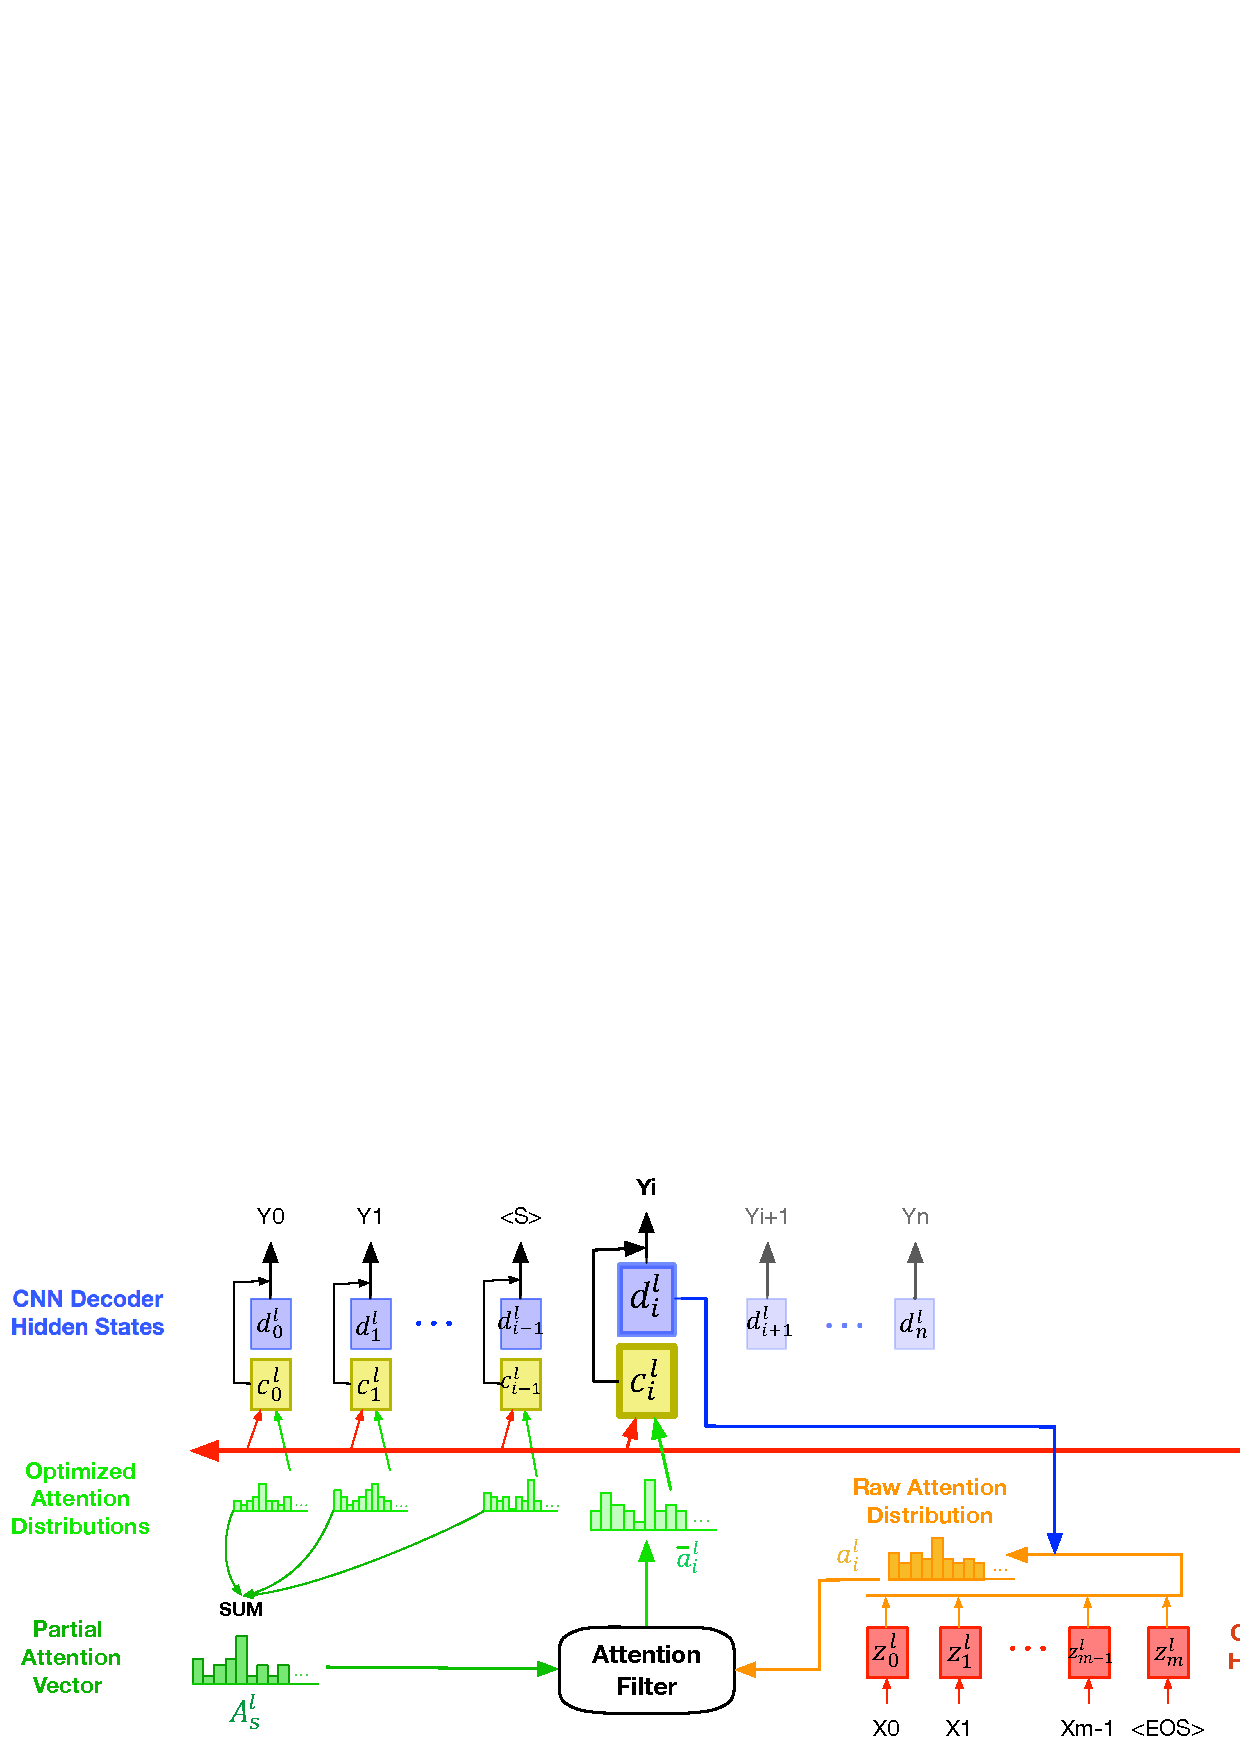
\includegraphics[width=0.85\linewidth]{model.pdf}
    \caption{The architacture of baseline model and pretrained model for keyword-aware extractor. $w$ represents words in corresponding sentences. $s$ represents sentence embeddings. $h_{SEP}$, $h_{EOD}$ and $k_{SEP}$ are three random initialized vectors for special tokens, which are updated during training.}
    \label{fig:model}
\end{figure*}

%In extractive summarization,
%We take the source document $D = (d_0, d_1, ..., d_n)$ and set-level 
%pseudo summary $P = (p_0, p_1,...,p_{m})$ as output.
%$d$ denote the sentence in source document.
%Each $p$ is a set of sentences.
%Our goal is that the selected sentences 
%from source document are the same as pseudo summary at sentence-level and set-level.

\textbf{Keywords Encoder.} 
We use TextRank algorithm to 
receive a sequential list of keywords 
%$K=(k^0_0,k^0_1,...,k^n_|K|)$ 
from the source document, 
ordered by their original positions in the source. 
%$k^i_j$ is the $j$-th keyword in $K$, which belongs to the $i$-th sentence in the source document. 
We take convolutional neural network (CNN) model to embed extracted keywords as $(\bf k_1, \bf k_2,..., \bf k_{|k|})$,
where $|K|$ is the number of keywords.
The combination of keywords representation and sentence representation
enbodies the intuition that the keywords are more important carriers of
the salient information and should be treated specially during sentence selection.
%of source document.

\textbf{Document Encoder.}
%In this work 
We consider two options for the document encoder:
training from scratch with \textit{BiLSTM document encoder} and fine-tuning on pretrained model named 
\textit{HIBERT document encoder}. 
The former is a standard document encoding model, and the latter is the state-of-the-art pretrained model for document encoding. 
%\KZ{Why only these two options?}

The \textit{BiLSTM document encoder} has two sub-encoders: a sentence encoder based on temporal CNN model and a document encoder based on bidirectional LSTM network. 
%A document is represented as $(\bf h_0,\bf h_1,...,\bf h_n)$ where $\bf h_i = [\overrightarrow{\bf h_i};\overleftarrow{\bf h_i}]$ is the representation of $i$-th sentence.
A document is represented as $(h_0,h_1,...,h_n)$ where $h_i = [\overrightarrow{h_i};\overleftarrow{h_i}]$ is the representation of $i$-th sentence.
%sentence encoder and document encoder.
%We take a temporal convolutional (CNN) model as sentence encoder which 
%gets sentence vectors of $D$ by encoding the word sequences. 
%%The CNN-based sentence vectors source document become $(s_0,s_1,...,s_n)$
%Then, we take these sentence vectors as the input to 
%a bidirectional LSTM network% which is the document encoder
%learning sentence representations given their surrounding sentences as context.
%The document representation based on BiLSTM encoder is represented as
%$(h_0, h_1,...,h_n)$,
%and the representation of $i$-th sentence is $h_i = [\overrightarrow{h_i};\overleftarrow{h_i}]$ 

%As the pretrained models can generate very strong sentence representations,
%we utilize the HIBERT encoder and fine-tune it on the training set 
%consisting of source documents and pseudo summaries.
%
The \textit{HIBERT document encoder} is a pretrained encoder~\cite{HiBert19},
which contains two Transformer-based sub-encoders.
We combine the word embeddings and their corresponding position embeddings as the input and obtain the context sensitive sentence
%representations $(\bf h'_0,\bf h'_1,...,\bf h'_n)$ as the output.
representations $(h'_0,h'_1,...,h'_n)$ as the output.
%to
%get the input vectors of sentence encoder.
%The sentence encoder transforms the inputs
%into a list of hidden representations $(x_0, x_1,...,x_{|d_i|})$. 
%We take the $t_i = x_{|d_i|}$
%as the representation of sentence $d_i$.
%The document encoder is a 
%Transformer applied on the sentence level.
%We obtain the context sensitive sentence representations $(h_0, h_1,...,h_n)$
%by running the Transformer on sentence representations 
%$(t_0, t_1,..., t_n)$, 

\textbf{Aligned Pointer Decoder.} 
%Based on the document representations and keywords representation from encoders,
We extend Pointer Network~\cite{PointNet15} as the decoder.
%to extract sentence from source document.
The pseudo summary consisting of multi-sentence sets is the input of the decoder.
%\KZ{What does supervised signal mean? Isn't it just the input to the decoder?}
We extract a set of keywords for each multi-sentence set in the pseudo summaries and 
order them based on their positions in the input text.
%The pseudo keywords also consists of 
%multi-keywords sets.
To distinguish the sentences and keywords in different sets, 
we set the representations for the
placeholder $<$SEP$>$ in pseudo summaries and pseudo keywords.
The pseudo summary becomes $P=(p^0_0,p^0_1,...,p^0_j,SEP,p^1_{j+1},...,P^m_x)$,
and its keywords become $K=(k^0_0,k^0_1,...k^0_j,SEP,k^1_{j+1},...,k^m_{|k|})$.
We randomly initialize the representation of $h_{SEP}$ for pseudo summary and $k_{SEP}$ for pseudo keywords. 

At each time step $t$, we take the output of decoder attending to the encoder sentence representations 
as the predicted vector $c^h_t$, which is calculated by:
%\KZ{I can't immediately relate the following formula to fig. 2.}
%\begin{small}
\begin{equation}
\small
\begin{aligned}
\small
c^h_t &= \sum_{i}^{n} {\alpha_{it}^h W^{a1} h_i} \\
\alpha_t^h &= \textup{softmax}(v^h \tanh(W^{g1} g_t + W^{h1} h_i)) \\ 
\end{aligned}
\end{equation}
%\end{small}
where $g_t$ is the decoder hidden state at step $t$.
$h_i$ is the sentence representation of $i$-th sentence
based on document encoder (BiLSTM or HIBERT).
$a_t^h$ is the attention weights based on sentences.
$W$ and $v$ in different labels are trainable parameters.
Similarly, the keywords vector $c_t^k$ can be computed.
%as follows:
%\begin{equation}
%\small
%c_t^e = \sum_{j}^{m} {\alpha_{jt}^e W^{a2} e_j} \\
%\end{equation}
%\begin{equation}
%\small
%\begin{aligned}
%c_t^e = \sum_{j}^{m} {\alpha_{jt}^e W^{a2} e_j} \\
%\alpha = softmax(a_t^e)
%a_{jt}^e = v^h \tanh(W^{r2} r_t + W^{e1} e_j) \\
%\end{aligned}
%\end{equation}
%where $h_i$ is the document representation of $i$-th sentence.
%Both $h_{SEP}$ and $e_{SEP}$ participate the calculation.

We compute the current extraction probabilities
using predicted sentence vector and keywords vector:
%\begin{small}
\begin{equation}
\small
\begin{aligned}
p(y_t|y_1,..,y_{t-1},c^h,c^k) = \textup{softmax}(v \tanh(W^{g} g_{t}  +& W^{h} c_t^h  \\
                                                     +& W^{k} c_t^k))
\end{aligned}
\end{equation}
%\end{small}
%where $y_t$ is the lable of sentence with the highest probability.
where $y_t$ is the sentence with the highest probability at current step.

\textbf{Combinatorial Loss.} 
We propose a combinatorial loss to train extractor, including
cross-entropy loss, keywords loss and set loss.
The {\em cross-entropy loss} reflects the accuracy of one-to-one alignment between
extracted sentences and pseudo summaries, which is computed as:
\begin{equation}
\small
L_{ce} = - \sum_{(P,D) \in T}{\log(p(P|D))}
\end{equation}
where $T$ is training set with $N$ samples.
We use {\em keywords loss} to emphasize the importance of the related salient information.
%can deal with the incorrect selection causing by
%the generated sentence representation which are similar to the 
%ground truth but without salience information based on keywords.
The probability of keywords extraction is computed as: 
%\begin{small}
\begin{equation}
\small
p(k_t|k_1,...,k_{t-1},c) = \textup{softmax}(v \tanh(W^{'g} g_{t} + W^{'k} c_t^k)) 
\end{equation}
%\end{small}
where $k_t$ is the predicted keyword at $t$ step.
We compute the keywords loss based on the keywords ground truth $K$ 
and source document $D$ as:
%\begin{small}
\begin{equation}
\small
L_{key} = - \sum_{(K,D) \in T}{\log(p(K|D))}
\end{equation}
%\end{small}
%\JQ{ambiguity: In order to abstract the extractor output consisting of multi-sentence sets
%to generate a final summary,}
As the output of extractor consists of multi-sentence sets,
we need correctly predict $<$SEP$>$ at the proper positions.
%of the right sentences in each set.
For each training sample, we obtain intermediate summary $Q$ 
extracted from source document $D$, 
yielded by greedily selecting sentence that maximizes the output
probability at each time step.
We align the $<$SEP$>$ of $P$ and $Q$
in the same position by padding or truncation 
the sequence of sentence labels in the set of $P$.
For example, given pseudo summary $P = (p_0,p_1,SEP,p_2,SEP)$ 
and extracted intermediate summary $Q = (q_0,SEP,q_1,q_2,SEP)$, we get aligned pseudo 
summary as 
$P' = (q_0,SEP,q_2,SEP,SEP)$.
We define the {\em set loss} function as:
\begin{equation}
\small
L_{set} = -  \sum_{(P',D) \in T}{\log(p(P'|D))}
\end{equation}
%where $Y$ is the predicted results of $D$.

We use the combinatorial loss as follows:
\begin{equation}
\label{func:loss}
\small
L_{cl} = \frac{1}{N} (\lambda_{c}L_{ce} + \lambda_{k}L_{key} + \lambda_{s}L_{set})
\end{equation}


\subsection{Abstractor}
\label{sec:abs}
The abstractor can paraphrase the inputs in parallel.
We take set-level pseudo summaries and their reference summaries 
as the input and output of abstractor at training.
%which is the pseudo summaries at training and the output of extractor at testing.
The abstractor is an independent neural network without parameter sharing with
the extractor.

In this work, we take two representative Enc-Dec model options 
as our abstractor: the standard Enc-Dec model PointerGen~\cite{SeeLM17} 
with attention mechanism~\cite{luong15} and copy mechanism,
%The copying mechanism help decoder
%replace the predicted word of out-of-vocabulary by
%the word with highest attention score in encoder.
%The embedding matrix
%as well as output projection matrix 
%words in the input document, follow by Paulus~\shortcite{PaulusXS17}. 
and a pretrained language model BART~\cite{BART19} 
finetuned on our pseudo summaries and reference summaries.
%consists of bidirectional transformer encoder and auto-Regressive transtormer decoder,
%it can be directly fine-tuned for abstractive summarization tasks and outperforms
%previous models. 

\textbf{Special loss.} For training, 
%we take pseudo summary $P$=($p_0$, $p_1$, ..., $p_t$, ..., $p_m$) as input
%we take pseudo summary $P$ consisting of multi-sentence set $p = (w_0,w_1,...,w_u)$ as input
%and merged reference summary $\hat{R}$ consisting of multi-sentence set $b = (w'_0,w'_1,...,w'_v)$ as output.
we take pseudo summary $P$ as input
and reorganized reference summary $\hat{R}$ as output.
%and its corresponding reference summary $B=(b_0,b_1,...,b_m)$ as output, 
%which respectively consist of multi-sentence set $p = (w_0,w_1,...,w_u)$ and $b = (w'_0,w'_1,...,w'_v)$.
%$w_u$ and $w'_v$ represent the word in the set of sentences.
%\KZ{Don't really understand the above... Why call it parallel loss? The abs are parallel so the loss is computed in parallel but calling it parallel loss is
%a bit strange i think. Also why bold the ``parallel loss.'' It's a bit out of
%place.}
%As our abstractor is paralleled, 
Given a pseudo summary, our abstractor deal with the sets in pseudo summary in parallel,
so we first compute the \textit{cross-entropy loss} between $i$-th multi-sentence set of 
pseudo summary and reference summary 
\begin{equation}
\small
L'_{ce}(i) = - \log(p(\hat{r}_i|p_i))
\end{equation}
Then, we consider all of the sets in a complete summary.
%The \textit{propotion of the loss} of $t$-th multi-sentence set over the complete summary is
%calculated as:
%\begin{equation}
%\small
%\label{func:abs_loss}
%PoL(t) = \frac{L'_{ce}(t)}{\sum_{t=0}^{m}{L'_{ce}(t)}}
%\end{equation}
%where $m$ is the number of sets in a pseudo summary, 
%denoting the number of the partitioned abstractor of parallelled abstractors.
%The loss of $t$-th abstractor in parallelled abstractors is as follows:
The loss of $i$-th set in pseudo summary is as follows:
\begin{equation}
\small
\begin{aligned}
\small
L_{sp}(i) = \frac{(1+PoL(i))}{2} L'_{ce}(i) \\
PoL(i) = \frac{L'_{ce}(i)}{\sum_{i=0}^{m}{L'_{ce}(i)}}
\end{aligned}
\end{equation}
where $PoL(i)$ is
\textit{propotion of the loss} of $i$-th sentence set over the complete summary.
This can strengthen the penalty for worse predicted multi-sentence set in a complete summary.

\subsection{Comprehensive Reinforcement Learning}
\label{sec:rl}
We apply comprehensive reinforcement learning (CRL) to make ext-abs framework an end-to-end trainable model.
%We pretrain the extractor and abstractor separately on (source document, pseudo summaries) pairs
%and (pseudo summaries, reference summaries) pairs.
%Then we fine-tune them on source documents and reference summaries through RL,
%which avoid abstractor training with irrelevant selected sentences
%and extractor with noisy reward.
We use policy gradient technique to optimize our model and take 
extractor as the RL agent.

During training, we first use extractor to obtain an 
intermediate summary $Q$, which is divided into several sentence sets by $<$SEP$>$.
Then, the abstractor paraphrases the sets in $Q$, 
and connects the rewritten sentences with $<$SEP$>$ to generate an abstractive summary $A$.
%The ROUGE scores between $<$SEP$>$ and other sentences are $0$.
%The extracted summary are divided into sentence sets by $<$SEP$>$,
%which .
%If the sentence is $<$SEP$>$, we set it as an empty sequence and take it as the end of the set. 
%\footnote{Given two sequence, if one of them is empty, the ROUGE score is $0$.
%If both are empty, the ROUGE score is $1$.}
%\JQ{soooooo many notations here. Why not move them to their corresponding 
%part and use it here directly.}
%The extracted summary $Q = (q_0^0,q_1^0,...,q_t^l,...,q_{y}^{M})$ and 
%its pseudo summary $P = (p_0^0,p_1^0,...,p_t^l,...,p_x^m)$ 
%consists of sentences.
%$A = (a_0,a_1,..,a_{M})$ is the generated abstractive summary of abstractor, 
%which summarized from the predicted pseudo summary $Q$.
%$B = (b_0,b_1,..,b_m)$ denotes reference summary corresponding to $P$.
%Both $A$ and $B$ consist of multi-sentence sets.
%$q_t^l$ means that the $t$-th sentence in summary belongs to the $l$-th sets.
%$m$ denotes the number of set in pseudo summary and reference summary.
At each time step $t$,
in order to compare the intermediate summary $Q$ and pseudo summary $P$,
we define a {\em sentence-level reward} using
ROUGE-L (R-L) score between the sets of $Q$ and $P$ at the same position.
\begin{equation}
\small
R_{sen}(t) = R\textup{-}L_{F1}(q_t,p_t)
\end{equation}
The sentence-level reward directly measures the accuracy of intermediate
summary sentences.
As the intermediate sentences and pseudo sentences are 
both extracted from source document,
the R-L, calculating the longest common subsequence (LCS), is the best way to 
evaluate the intermediate sentences with the 
pseudo sentences.

To evaluate the alignment between intermediate summary $Q$ and 
reorganized reference summary $\hat{R}$, we propose a {\em set-level reward}.
%The ground truth pseudo summary should be padded (truncated) as $P'$ in {\em set loss}, 
%For example, given
%predicted pseudo summary $Q=(q^0_0,q^0_1,q^0_2,SEP,q^1_3)$ and ground truth pseudo summary $P=(p^0_0,p^0_1,SEP,p^1_2,p^1_3,SEP,p^2_4)$,
%the number of sets in merged reference summary $\hat{R}=(\hat{r}^0,SEP,\hat{r}^1,SEP,\hat{r}^2)$ is the same as $P$.
%$\hat{r}^l$ is the concatenation of the sentences in $l$-th set of $\hat{R}$.
%For the set-level comparsion, we align the $SEP$ in $Q$ and $P$ by truncating the larger set of $Q$ and $P$.
%Thus, the processed pseudo summary become $(q^0_0,q_^0_1,SEP,q^1_3)$ and $(p^0_0,p^0_1,SEP,p^1_2)$.
We compute the {\em set-level reward} by ROUGE-2 (R-2) as:
\begin{equation}
\small
R_{set}(t) = 
	\begin{cases}
		   \mbox{$R$-$2_{recall}(a^l,\hat{r}^l)$}, \quad \quad \mbox{if $t=b+|q^l|$}\\
           \mbox{$R$-}2_{recall}(\mbox{concat}(q_b^l...q_t^l),\hat{r}_l), \quad    \mbox{otherwise}\\
   \end{cases}
\end{equation}
%where $seq$ connect all the inputs together.
where $concat$ concatenates all the inputs.
$\hat{r}^l$ is the $l$-th set of sentences in $\hat{R}$ and $|q^l|$ is the number of sentences in $l$-th set of $Q$.
$b$ is the index of the first sentence of $l$-th set in $Q$.
$t=b+|q^l|$ means that the prediction of $l$-th set in intermediate summary is over.
For {\em set-level reward}, at step $t$, we concatenate all of the extracted sentences in $l$-th set as a extracted set $E_t^l$ 
and compute the R-2 score between $E^l_t$ and its corresponding set $\hat{r}^l$ in reorganized reference summary.
At the end of the prediction of this set, we compare the abstractive summary $a_l$ generated from $q^l$ with $\hat{r}^l$.
Since reference summary is abstractive which has many variant, the R-2 matching bigram between summaries is more suitable.
As the $E_t^l$ is the part of the input of the abstractor, the ROUGE score reflects the alignment between the input and output of abstractor 
during test.
The higher recall between $E_t^l$ and $\hat{r}^l$
means that the $E_t^l$ contains more information of $\hat{r}^l$ and can predict better abstractive summary.
%The recall can reflects the coverage of reference summary.
%We use R-2 to evaluate the alignment between extracted sentences and merged reference summary


Considering the quality of an overall generated summary,
we compute {\em summary-level reward} as:

\begin{equation}
\small
R_{sum}(t) = 
	\begin{cases}
		   \mbox{$R$-$2_{F1}(\mbox{concat}(a^0...a^l), \mbox{concat}(\hat{r}^0...\hat{r}^l))$}, \mbox{if $t=\sum\limits_{0}^{l}|q^l|$}&\\
           \mbox{$R$-}2_{F1}(\mbox{concat}(q_0^0...q_t^l), R), \quad \mbox{otherwise}&\\
   \end{cases}
\end{equation}
where $t=\sum\limits_{0}^{l}|q^l|$ means that prediction of $l$-th set in 
intermediate summary is over.
For {\em summary-level reward}, we concatenate all of the extracted sentences as a extracted set $E_t$ at each time step $t$.
We use F1 score as reward, because the length should be considered during evaluating the whole generated summary,
which can also reflects the alignment of abstrator.
At the end of the prediction of each set, we compare the concatenated generated abstractive summary and corresponding
reference summary. 
Especially, while the prediction of model is over, we compute the R-2 F1 score between generated abstractive summary $A$ and reference summary $R$.

The total reward is the combination of above:

\begin{equation}
\label{func:reward}
\small
R_{overall} = \gamma_{1}R_{sen} + \gamma_{2}R_{set} + \gamma_{3}R_{sum}
\end{equation}



